\documentclass[tikz,border=5pt]{standalone}
\usepackage{pgfplots}
\pgfplotsset{compat=1.18}
\definecolor{corba}{HTML}{3F51B5}\definecolor{punt}{HTML}{D32F2F}
\begin{document}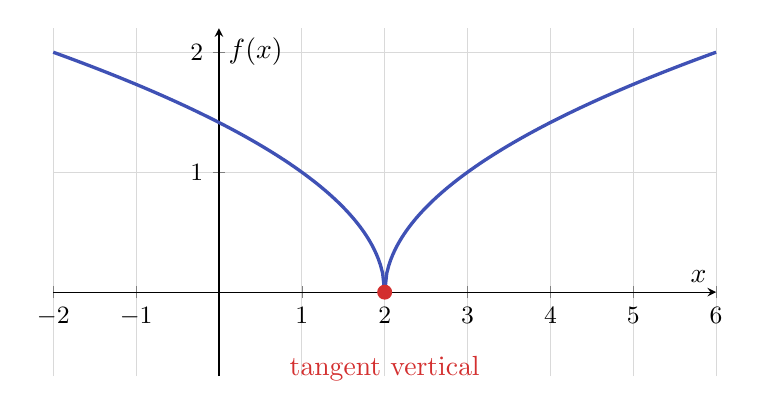
\begin{tikzpicture}
\begin{axis}[width=10cm,height=6cm,axis lines=middle,xmin=-2,xmax=6,ymin=-0.7,ymax=2.2,
 xlabel={$x$},ylabel={$f(x)$},grid=major,grid style={black!15},tick label style={font=\small},clip=false]
 \addplot[corba,very thick,domain=-2:2,samples=160]{sqrt(2-x)};
 \addplot[corba,very thick,domain=2:6,samples=160]{sqrt(x-2)};
 \addplot[only marks,mark=*,mark size=2.5pt,punt] coordinates {(2,0)};
 \node[anchor=north,font=\normalsize,text=punt] at (axis cs:2,-0.45) {tangent vertical};
\end{axis}\end{tikzpicture}\end{document}
